% !TEX root =  paper.tex
% \newpage
% \  \ 
% \newpage
\section{Proposed Approach}
\label{sec:approach}

The proposed approach performs web page segmentation 
based on visual analysis of the page.
Existing state-of-the-art techniques (e.g., VIPS~\cite{cai2003vips}) 
are heavily based on DOM information (e.g., element tree relationships) 
with a few visual attributes.
In contrast, our approach performs an extensive visual analysis that examines
the overall visual structure and layout of the page, 
and therefore aims to more faithfully capture the visual structure of the page as 
would be perceived by a human user, as opposed to heavily relying on how the 
elements are structured in the DOM. 
While the proposed approach is chiefly visual in nature,
it does combine aspects of both the DOM and visual page analysis 
in a fashion that aims to minimize the drawbacks of each approach, 
which were described in \Cref{sec:background}.
The approach is also parameter-free,
requiring no thresholds for its operation and therefore
reduces the manual effort required and
makes the accuracy of the approach
independent of manual parameter tuning. 

\Cref{fig:approach-overview} shows an overview of the proposed approach.
The approach begins by retrieving the DOM 
of the rendered page.
Next, unlike techniques that are heavily based on DOM hierarchy and other DOM attributes, 
we only use a few key nodes of the DOM (as described in \Cref{subsec:abstraction}) 
and discard the rest of the tree.
The output of this process is a normalized and abstract representation of the page.
This transforms the page into a set of \vizobjs,
each of which represents a basic unit of visual information 
(e.g., a text, an image).
The approach then extracts features from these \vizobjs,
consisting of both DOM features as well as visual features.
Finally, the objects are grouped using unsupervised machine learning clustering
and the relevant DOM nodes are finally extracted as segments of the page.

\begin{figure}
    \centering
    {%
    \setlength{\fboxsep}{0pt}%
    \setlength{\fboxrule}{1pt}%
    \fbox{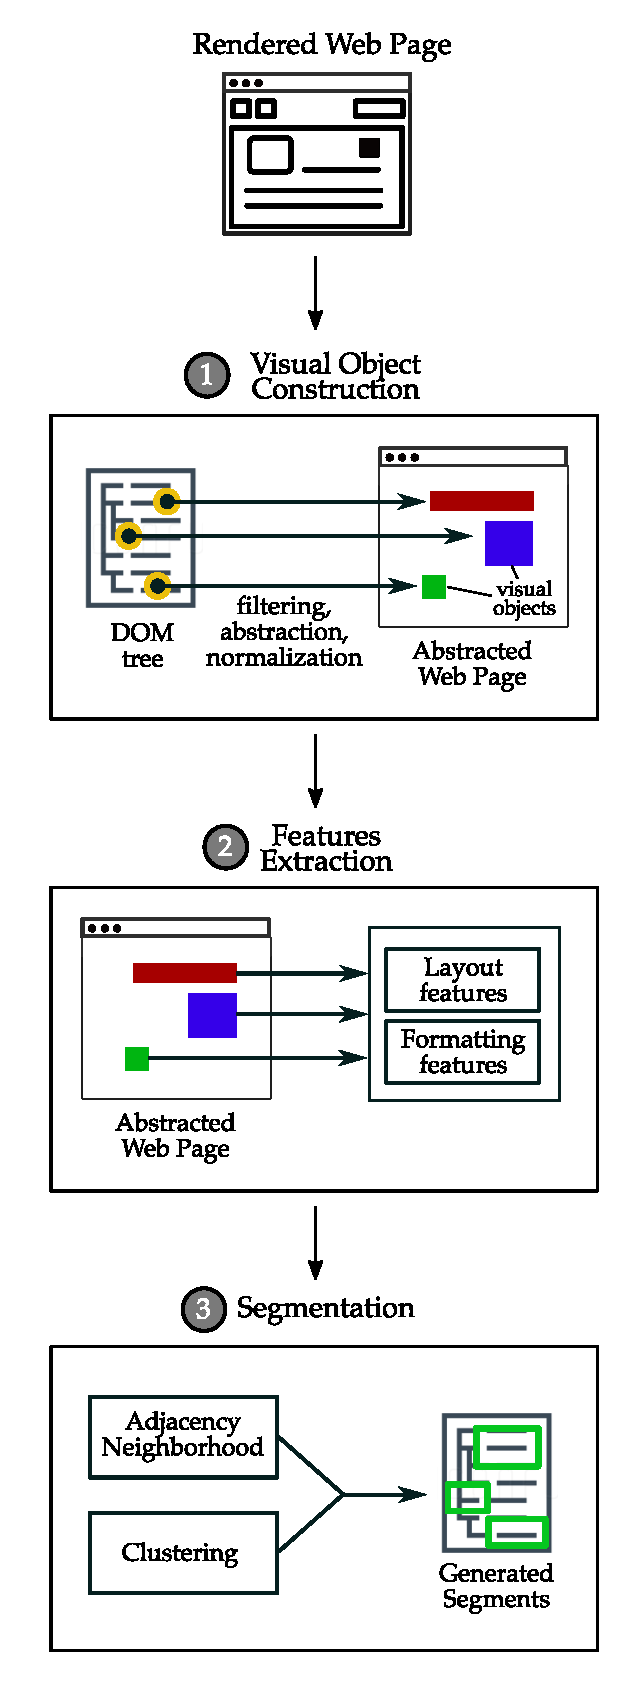
\includegraphics[trim=0 0 0 0,clip,scale=0.6]{figures/approach/approach.pdf}}
    }%
    \caption{Overview of the proposed approach.}
    \label{fig:approach-overview}
\end{figure}

In the following subsections,
we describe each step of the proposed approach
and illustrate their major components and analysis procedures.

\subsection{Visual Object Abstraction}
\label{subsec:abstraction}
In the first step of the approach,
we take as input the DOM of the page
after it is loaded and rendered in a browser.
We then perform a \emph{visual abstraction} that 
transforms the DOM into a set of \emph{\vizobjs},
which are visual abstractions of the visible subset of DOM elements.
Each {\vizobj} contains only the location and type an element.
All other information is removed. This is contrast to techniques 
that are heavily DOM-based (e.g., VIPS), which rely on DOM hierarchy 
traversal at every step of their analysis.

The rationale for this abstraction step is as follows.
First, by performing an abstraction
we aim to normalize the rendering of a page
into an abstract representation 
that signifies the salient features of the page
from a visual perspective.
The intuition behind this is that
normalization and abstraction can be helpful to 
achieve our goal of detecting segments, 
since the exact and minute page rendering details
are less relevant when aiming to divide the page as a whole
into a set of segments. 
Therefore, this visual object abstraction stage
enables obtaining a big picture overview of the page
to identify such commonalities despite minute differences.

% Furthermore,
% there is evidence that humans represent objects in an abstract way 
% before visually analyzing their grouping~\cite{humphreys2017visual, feldman2003visual}.
% That is, the details of the object (i.e., the actual picture of an image element, the meaning of a text)
% are abstracted away in favor of higher level information 
% (i.e., that it's type is a text, that it is located in a certain region).
% Our visual object abstraction behaves in the same way,
% by removing all details of the object except for high level information such as object type and location.
% % The abstraction allows the brain to easily identify similarities 
% % between various instances of an object as well as recognizing various
% % visual data as belonging to a group.

The visual object abstraction is implemented as follows.
First, we extract from the DOM a set of nodes that 
represent visual content of the page, 
and we refer to each of these as \emph{{\VizObjs}}.
We define three types of {\VizObjs}:
textual, image, and interactive.

\header{Textual Objects}
The extraction of text content is achieved by 
traversing text nodes of the DOM. More specifically:
\begin{align}
    \Theta_{t} \coloneqq \{ E \:\vert\: \nu(E) \land \tau(E) \}
\end{align}
where $\Theta_{t}$ is the set of all {\vizobjs} that represent text in the page,
$E \in DOM$ is a leaf element iterator of the rendered DOM in the browser,
$\nu(E)$ is a heuristic predicate that runs a series of checks
to detect visible elements,
and $\tau(E)$ is a predicate that examines whether
there is a text associated with $E$. 
More specifically, it returns
non-empty nodes of DOM type \code{\#TEXT},
which represent string literals. 
We note that the predicate is based on a node type, rather than
an element (i.e., tag) type.
This allows more robust abstraction because the predicate captures any text and does not
make assumptions about how developers choose to place their text.
In other words, regardless of the tag used for text data (e.g., \code{<span>, <div>}),
text would still be stored in nodes of type \code{\#TEXT}, even for custom HTML elements.
This helps in making the approach more robust by reducing assumptions about
tags and how they are used in the page. 


\header{Image Objects}
Subsequently, we perform another extraction for image content.
We define this as follows:
\begin{align}
    \Theta_{m} \coloneqq \{ E \:\vert\: \nu(E) \land \mu(E) \}
\end{align}
where $\Theta_{m}$ is the set of all {\vizobjs} that represent images.
As in the previous case,
the predicate $\mu(E)$ examines whether
there is any relevant image content associated with $E$.
This has two possibilities:
nodes of \code{<img>}, \code{<svg>}, and \code{<canvas>} elements, 
and non-image nodes with a non-null background image.
We note that this predicate makes the proposed approach more robust
by eliminating assumptions about how developers choose to add images.
If images are contained in standard image tags (e.g., \code{<img>}, \code{<svg>}),
then our predicate readily captures those elements.
However, we make no assumptions that this is the only way an image can be included.
For this reason, we also capture elements of any tag type when we detect a non-null background image.

\header{Interaction Objects}
Finally, we extract the interaction elements as follows:
\begin{align}
    \Theta_{i} \coloneqq \{ E \:\vert\: \nu(E) \land \eta(E) \}
\end{align}
where $\Theta_{i}$ is the set of all {\vizobjs} that represent form elements or similar interactive elements.
These are determined by the predicate $\eta(E)$, which collects
elements such as input fields and drop down menus.

We finally obtain the total set of {\vizobjs}
in the page, $\Omega$:
\begin{align}
\Omega = \left( \Theta_t \cup \Theta_m \cup \Theta_i \right)
\end{align}

We now make a number of remarks about the abstraction process.
We use a DOM approach instead of a visual approach 
for this abstraction step for the following reasons.
While visual techniques might be useful for analyzing
the visual structure of a page since 
they mimic what a human user would be seeing,
they can be at a disadvantage in some tasks.
For instance, identifying textual objects using a visual approach is based on OCR (optical character recognition),
which involves analyzing image pixels and detecting wether or not the pixels constitute a text.
OCR remains a challenging and active area of research in the computer vision community.
The same task (i.e., identifying textual objects) 
is readily available and immediately accessible from the DOM, 
and therefore DOM-based approaches would be more suitable for this task.

Furthermore, while state-of-the-art techniques (e.g., VIPS~\cite{cai2003vips})
rely heavily on the DOM tree by traversing all elements of the tree and checking for various rules and heuristics
between parents, children, and other nodes, our approach is agnostic to the DOM tree.
Our approach does not traverse the elements of the tree and does not check for relationships between any nodes.
The approach only accesses a subset of leaf nodes, and only gets basic information from those nodes, such as node type.
The approach is therefore only loosely related to leaf nodes and agnostic to the DOM tree itself.
This observation, coupled with the fact that we use visual analysis for the remaining steps of the approach,
minimizes some of the drawbacks of DOM-based approaches mentioned in \Cref{sec:background},
such as the fact that they are not directly related
to what the user is actually perceiving on the screen.


\subsection{Features Extraction}
So far, the DOM has been
abstracted and a set of {\vizobjs} were constructed.
We now proceed by defining a mechanism to utilize these {\vizobjs}
and build on them to construct the final page segments,
which are the end goal of our proposed approach.
Accordingly, in this stage we transform each {\vizobj} constructed
in the previous stage into a feature vector.
This acts as a dimensionality reduction step
in which the {\vizobjs} are further abstracted to facilitate
reasoning and analysis. This will then be used
in subsequent stages to segment the page.

% At this feature extraction stage,
% we again utilize cues from the human brain's visual cognition system.
% Studies have indicated that,
% among other factors,
% the brain relies on cues of location, color, and continuation
% (i.e., alignments) \cite{feldman2003visual,humphreys2017visual,palmer1994rethinking}.
% These cues allow the brain to perceive 
% visual stimuli as belonging to the same object.
% We hence adopt this aspect of cognitive processing and 
% build a feature vector containing these cues.
% The features will be used in a later stage to finally
% create page segments.

We now describe the details of extracting the feature vector, 
which consists of the location, dimensions, foreground color, and background color
of each \vizobj. 
First, we extract spatial data.
We capture the x and y coordinates of the CSS box model of the \vizobj.
These are not the coordinates as defined in the DOM attributes,
but rather the \emph{computed} coordinates, as rendered by the browser.
This represents the final absolute (relative to the viewport) location
of the final rendered elements, in order to more faithfully capture the 
final visual representation as seen by the user.
We also capture the computed width and height of the box model in the same fashion.
%
Next, we extract color information for the \vizobjs.
Two color values are captured: background and foreground colors.
These colors are obtained through a combination of computed DOM style
values as well as computer vision methods.
The definition of these values depends on the type of the \vizobj.
For all object types, 
the background color is computed through computer vision.
The value of the background color is set to the value of the color mode 
of the region surrounding the box model. 
We use computer vision because DOM colors are declarative in nature
and do not capture the actual final rendered pixels on screen.
For instance, the computed style may indicate that the background
is transparent, while the final rendered color might actually end up being 
not transparent due to interactions with other elements of the DOM. 
This results in a situation where the computed style of 
the element itself can not be used to determine the actual rendered style.
Therefore, we use computer vision as the ultimate source of truth for 
information on the final rendered image.
For text and input objects, the foreground color is obtained from
the computed DOM style as it faithfully represents the image rendering.
For image objects, the foreground color is computed as
the color mode of the region contained inside the object's box model. 

\subsection{Page Segment Generation}

\header{Adjacency Neighborhood Construction}
In order to start analyzing the extracted {\vizobjs} features
and build page segments, we define some notion of 
adjacency information.
Adjacent objects are more likely (but not necessarily) to belong
to the same segment, and therefore it would be beneficial
to obtain some form of \emph{adjacency neighborhood} for 
the \vizobjs.
Whether or not adjacent objects actually
end up belonging to the same segment depends on the rest of the features.

The adjacency neighborhood is a data structure that captures the spatial visual layout grouping 
of the objects as rendered on the page. 
We build adjacency information using the computational geometry~\cite{toth2017handbook}
techniques often used in computer vision, which perform extensive analysis 
of how objects are overlaid with respect to each other and provide
information about their neighborhood.
The adjacency neighborhood would then be used at a later stage
to guide the unsupervised clustering process.

% We perform this step to model the brain's visual cognitive processing.
% It has been shown that spatial proximity is a strong factor
% in the brain's visual cognition when performing
% a perceptual grouping of objects
% ~\cite{palmer1994rethinking, palmeri2004visual}.
% Visual stimuli that are in close proximity to one another
% are registered in the brain as bearing more potential for grouping.
% Therefore, in this stage we model this processing mechanism in the brain
% by means of a neighborhood analysis of the extracted {\vizobjs}.

We now precisely define the adjacency neighborhood 
and the process of constructing it.
We begin by populating a spatial index from the coordinates
of {\vizobjs}.
A spatial index~\cite{beckmann1990r}
is a data structure that facilitates querying spatial relationships
between the contents of the index.
We therefore use the spatial index to resolve spatial queries and
construct an adjacency neighborhood for the extracted objects.
More concretely, we define the adjacency for {\vizobjs} as follows:
\begin{equation}
\alpha(o) \coloneqq \{ n \in \eta(o) \:\vert\: \eta(o) \cap \lambda(o, n) = \varnothing \}
\end{equation}
where $\alpha(o)$ is the adjacency neighborhood of the object $o$,
$\eta(o)$ is the nearest neighbors list of objects with respect to $o$,
and $\lambda(o, n)$ is the minimum distance line joining $o$ and $n$.
The equation computes the adjacency to $o$
where there is a direct non-intersecting 
visual line of sight with a neighbor.
This is achieved whenever the intersection of $\lambda(o, n)$
and the neighborhood $\eta(o)$ is the empty set as shown in the equation.
The end result is a set of objects comprising the
adjacency neighborhood of object $o$.


\header{Contextual Features Clustering}
Up to this point, we have
transformed the page into a set of {\vizobjs},
extracted relevant features from each object,
and constructed the adjacency neighborhood.
In this stage, we combine the adjacency neighborhood and
the feature vector to perform a \emph{contextual} features clustering.
In this process, we devise a variation of unsupervised clustering
that uses adjacency neighborhood as a context.
The rationale for this is that there will likely be a reduction in 
false positives and negatives if we were to localize the clustering
process to the adjacency.
We now describe the process by which we achieve this contextualization.

First, we analyze the adjacency neighborhood to extract a number of
\emph{scaling} factors.
These scaling factors guide the clustering towards using
the adjacency neighborhood as its context.
In other words, these factors can be thought of as adaptive thresholds 
that are automatically determined based on the data in order to 
better guide the clustering process.
More concretely, we have:
\begin{align}
    \sigma_D \coloneqq &\argmax_{\delta \,\in\, \Delta} \: \delta f(\delta) \\
    \mathrm{s.t.}& \:\: \Delta \coloneqq \{ d(o, n) \:\:\forall\:\: n \in \alpha(o), o \in \Omega\} \nonumber
\end{align}
where $\sigma_D$ is the \emph{distance factor},
$\Delta$ is the set of all pair-wise Euclidean distances, $d(o, n)$,
within all adjacency neighborhoods.
$n \in \alpha(o)$ is a member of the adjacency neighborhood of object $o$,
and $f(\delta)$ is the statistical frequency of the distance $\delta \in \Delta$.
The $\sigma_D$ factor represents the spatial distance density that matches
all clusters of adjacency neighborhoods.
In other words, the equation computes a \emph{weighted} statistical mode 
of pair-wise distances (restricted to adjacency neighborhoods).
This yields a distance value that represents 
the most probable spatial threshold of adjacency neighborhoods.
This factor $\sigma_D$ will be used in subsequent steps to guide the unsupervised clustering
in a parameter-free fashion. We now proceed to computing the next factor:
\begin{align}
    \sigma_A \coloneqq &\argmax_{\epsilon \,\in\, \Upsilon} \: \frac{f(\epsilon)}{\epsilon} \\
    \mathrm{s.t.}& \:\: \Upsilon \coloneqq \{ e(o, n) \:\:\forall\:\: n \in \alpha(o), o \in \Omega\} \nonumber
\end{align}
where $\sigma_A$ is the \emph{alignment factor},
$\Upsilon$ is the set of all pair-wise minimal alignment differences, $e(o, n)$,
within all adjacency neighborhoods.
$e(o, n)$ measures the smallest alignment differences between the pairs $o$ and $n$. 
It measures all potential alignment arrangements, such as left aligned, top aligned,
or center aligned objects. 
The equation measures a weighted statistical mode of all pair-wise
alignments in the adjacency neighborhood.
It optimizes alignment values that are as small as possible with as high
statistical frequency as possible.
This represents the scale of alignment between objects within adjacency neighborhoods.
% At this point, we reemphasize that the rationale for incorporating alignment
% measurements is to attempt modeling the brain's visual cognition.
% It is well known from cognitive science~\cite{pizlo1997curve,feldman1997curvilinearity}
% that the brain takes strong cues from the alignment of visual stimuli,
% and uses these cues to detect object grouping.
% We therefore believe that adopting similar cues can potentially be helpful
% for detecting page segments.

We now describe how $\sigma_A$ and $\sigma_D$ will be used to localize the clustering.
\begin{align}
D(o_A, o_B) \coloneqq \, S_D \: S_A \: \kappa(o_A, o_B)
\end{align}
where $S_D = f(\sigma_D)$ and $S_A = f(\sigma_A)$ are piece-wise functions
that clamp all distances below $\sigma_D$ and $\sigma_A$, respectively, to unity,
while keeping all other distances intact.
$\kappa(o_A, o_B)$ measures the perceptual differences in
background and foreground colors between the $o_A$ and $o_B$ using 
the CIE76 $\Delta{E}$~\cite{klein2010industrial} metric.
We chose this metric because it performs a comparison that takes into account
human visual perception of color, and therefore using this metric enables 
our approach to more faithfully mimic how a human would perceive the color.
Finally, the distance $D(o_A, o_B)$ is clustered using a density-based
clusterer (e.g., DBSCAN~\cite{ester1996density}).
Due to the scaling factors $\sigma_D$ and $\sigma_A$ that we have computed,
the density parameter for clustering simply becomes unity.
Once the clusters are obtained,
we retrieve the list of elements in each cluster, and
obtain their xpaths.
Each set of xpaths is finally reported as a segment
of the page and returned as the final output.

\subsection{Implementation}
We implemented the approach in a tool,
which we have called \toolname in reference to the brain's
cerebral cortex that plays a key role in perception and attention.
\toolname is implemented in Java.
We use the Selenium web driver to render the page in Google Chrome
and extract DOM trees and their relevant computed properties.
OpenCV is used for computer vision operations.
We also use the Apache Commons Math library for clustering and other
mathematical and numerical functions.
To make the study replicable, we have made {\toolname}'s source code 
and evaluation subjects available online~\cite{tool-and-data}.
